\section{Getting Started}
\subsection{Register an account}
\par{Users will have to visit \href{https://github.com/SpheMalo/COS-301-Main-Project}{\textbf{Figbook}} and click on 'Register'. The following will appear. }

\begin{figure}[h]
	\centering
	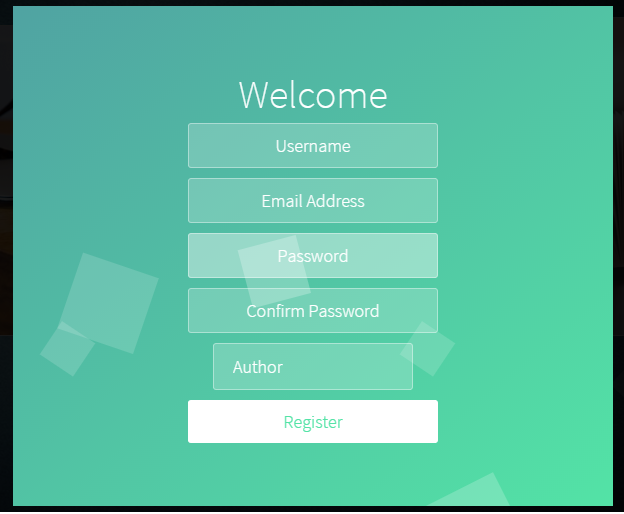
\includegraphics[width=200px]{images/register.png}
	\caption{Register screen of website}
\end{figure}

\par{Enter all requested information. The last field (before the 'Register' key) is a drop down key to select what role you'll play in the world of figbook. Different roles have different functionality so choose wisely. \\ Click on 'Register' and await confirmation.\\ \\ If any error occurs ('email address already exists' for example), try entering your details again (paying careful attention to spelling) or try enter different credentials.



\subsection{Log in}
\par{If you already have an account, go to \href{https://github.com/SpheMalo/COS-301-Main-Project}{\textbf{Figbook}} and click on the 'Log in' button. }

\begin{figure}[h]
	\centering
	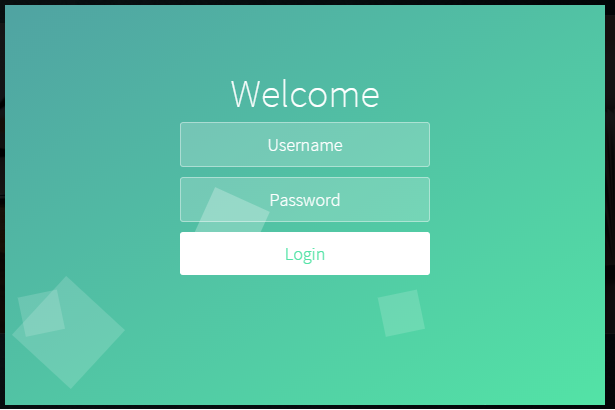
\includegraphics[width=200px]{images/login.png}
	\caption{Login screen of the website}
\end{figure}

\par{Enter either your username or email address (that you entered when you registered) and click 'log in'. If you have an existing account, you will be successfully logged in to the system.\\ \\ If you have no account, see the section above this one before continuing.}
\\
